\chapter{Introduzione}
\section{Cos'è il lettering}
La disciplina del lettering si può vedere come un punto intermedio tra due altre materie della grafica: \hl{calligrafia} e \hl{tipografia}.
\subsection{Calligrafia}
con calligrafia si intende \hl{l'arte della bella scrittura}, l'uso di strumenti e tecniche per la creazione e imitazione di caratteri storici. L'obiettivo primo della calligrafia è quindi unire caratteri ed estetica, oltre che comunicare qualcosa con i questi ultimi.

\begin{mdframed}[style=mystyle,frametitle=]
Quindi parola chiave: \hl{espressività ed estetica}
\end{mdframed}

\subsection{Tipografia}
con tipografia si intende la progettazione di \hl{caratteri volti alla stampa}, e nello specifico alla creazione di lettere e segni che siano funzionali e ottimali appunto una volta stampati. \textbf{Alla base c'è comunque un lavoro manuale di un designer} che abbozza e progetta i tratti delle lettere.

\begin{mdframed}[style=mystyle,frametitle=]
 Quindi parola chiave: \hl{funzionalità}
 \end{mdframed}

 \subsection{Lettering}
il lettering è invece un ibrido tra queste due discipline legate ai caratteri; infatti, nonostante nel lettering le lettere vengono disegnate a mano libero, il tutto è volto alla gestione delle scritture.
\begin{mdframed}[style=mystyle,frametitle=]
 Quindi \hl{lettering = punto intermedio tra calligrafia e tipografia}
 \end{mdframed}


\section{Enzo Mari | Design e formalismo | VIDEO}\label{sec-mari}
\begin{fancyquotes}
{\huge \textit{Tutto ciò che ci circonda, sia naturale che artificiale, è forma.Il problema della forma è ricercarne la sua essenza.} }

    
    La forma corrisponde al significato di un oggetto, alla ragione per cui un oggetto viene costruito e rappresenta, se è ben fatta, la sua più alta qualità. 
\end{fancyquotes}

Per fare un piccolo incipit, Mari, durante la sua carriera, è sempre andato alla ricerca dell' +\hl{essenzialità e funzionalità}, distaccandosi da tutto il superfluo e l'eccesso che nel corso degli anni si è sempre più ricercato, e spesso Mari usa provocazioni più o meno dirette per sottolineare il suo modo di pensare (come si nota anche dal video)  



\begin{wrapfigure}{l}{0.25\textwidth} %this figure will be at the right
    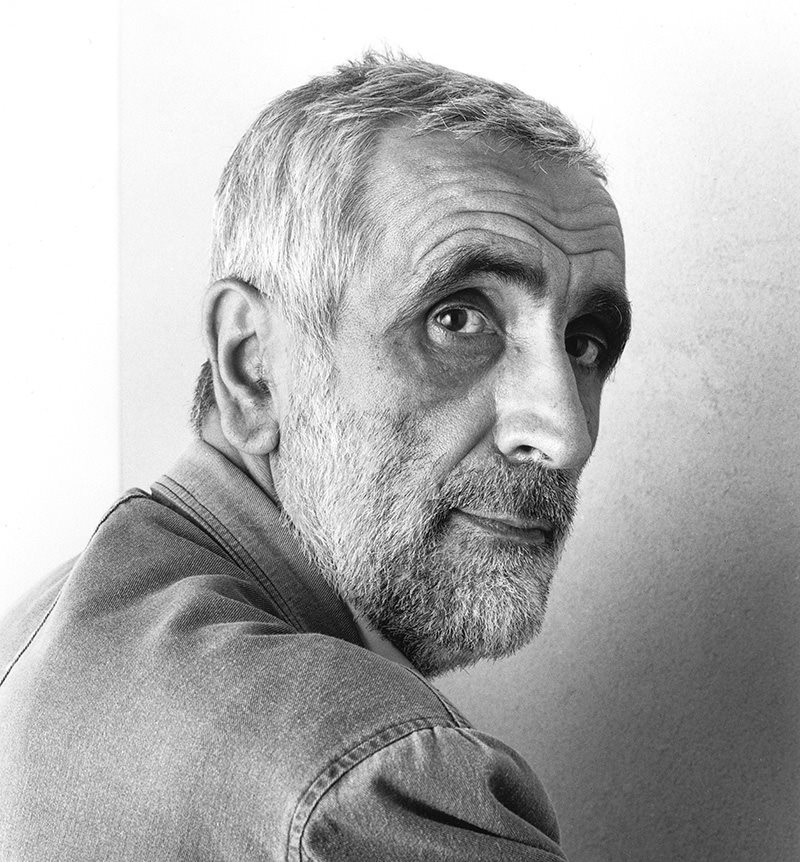
\includegraphics[width=0.2\textwidth]{blocco_1 - introduzione al corso/imgs/mari.jpg}
\end{wrapfigure}
Secondo Mari, \hl{esiste uno stretto legame tra funzione e forma di un oggetto}: ogni elemento che ci circonda, per svolgere la sua funzione, necessita di una forma, la sua \hl{forma essenziale}.
Il problema, però, è che esiste la tendenza ad "appesantire" l'essenzialità per ricercarne l'estetica, quando tutto ciò è assolutamente superfluo, \textbf{se non controproducente}.
Questa tendenza viene chiamata, da Mari, \hl{formalismo}, e gli oggetti/elementi realizzati in questo modo prendono il nome di  \hl{oggetti formalistici}.\\

\subsection{Formalismo}
Con formalismo si intende andare a rovinare quella che è la forma necessaria allo svolgimento di una funzione per fini inutili. E questa tendenza non è riferita solo ad esclusivamente al design, ma, come dice Mari, è un concetto applicabile a moltissimi campi.

Mari fa l'esempio degli arredi sfarzosi stile 800: gambe dei tavoli con zampe di leone, ricami particolarmente elaborati...tutti dettagli che vanno a stratificarsi sopra la forma essenziale del tavolo, e che lo rendono una \hl{forma sbagliata}

\begin{mdframed}[style=mystyle,frametitle=il formalismo è ignorante]
 Mari, sempre in maniera molto diretta, definisce il formalismo come \hl{ignorante}, nel senso che, a tutti gli effetti, ciò che fa è IGNORARE la ricerca dell'essenzialità legata alla funzionalità, appesantendo con l'inutilità
 \end{mdframed}

\subsection{Richiamo alla classicità}
Mari parla delle popolazioni classiche elogiando la loro visione; nel passato, infatti, Greci e Romani si ispiravano molto \textbf{guardando la natura}, ma non perchè fosse bella, ma perchè \hl{la natura, nelle sue forme, è sempre perfetta e giusta}: ogni elemento è lì perchè ha una suo funzione, e non è accompagnato da inutilità

\subsection{Contro il design moderno}
Secondo Mari, il fine ultimo del design moderno è quello di proporre oggetti e progetti che siano diverse in qualcosa rispetto a quelli già commercializzati; questa è la ragione per cui la quasi totalità degli oggetti moderni è formalistico.

Formalismo è ignorante

\subsection{Riconoscere un oggetto formalistico}
per capire se un oggetto è formalistico o no, basta ragionare se è possibile creare forme alternative di quest'ultimo; se è possibile, allora l'oggetto è formalistico, altrimenti è essenziale e corretto. Questo perchè, un oggetto GIUSTO, nella sua forma essenziale, non può presentare forme alternative: ha una sola forma, perchè la funzione che deve svolgere è quella

\subsection{Divano-letto fallimentare}
Tra i vari progetti portati a termine, quello del divano letto fu fallimentare: seppur aveva fatto centro sull'esigenza della popolazione (prezzo molto basso rispetto alla media, siamo nel periodo delle crisi abitative, la gente non aveva molti soldi), i rivenditori si rifiutarono di prenderlo per venderlo, perchè a loro avviso era troppo semplice, senza alcuna estetica e qualità percepita bassa, e nessuno l'avrebbe mai comprato.
\subsubsection{INCOMPRENSIONE}
Un tema importantissimo che nasce da questo fallimento è il fatto di non venir compresi. 

\hl{Nel mondo del design, ma anche in altri, bisogna fare i conti con la percezione esterna: magari un progetto a cui hai dedicato anima e corpo, sembra perfetto, la gente lo percepisce in maniera errata e lo fa diventare un flop}.
Purtroppo questo fa parte del gioco!

\subsection{Rendere la gente consapevole | Il progetto personale}
Non riuscendo a farsi comprende, Mari, capisce che una soluzione all'incomprensione è cercare di "educare" la gente, per portarla a capire la sua visione.

Decide quindi di proporre qualcosa di alternativo: è la gente che deve costruire l'oggetto d'arredo di cui necessita, per capire ciò che sta dietro.

Propone quindi una serie di arredi "a pezzi", che dovevano poi essere assemblati dai clienti; durante la presentazione viene addirittura accusato di fascismo (il design, secondo le credenze, doveva facilitare la vita, non sfruttare la gente per lavorare ulteriormente).

Nonostante ciò, la vendita funziona e Mari riceve molti complimenti, che però non lo rendono contento, perchè alcuni di essi non apprezzava l'idea dietro prodotto, bensì la sua "rusticità".

Di fatto, con questo progetto, però, ha anticipato di decenni la linea produttiva di grandissime realtà mondiali moderne come IKEA: commercializzare assi e aste di legno pre-tagliate, per poi lasciare al cliente la fase di assemblaggio.
\subsection{Insegnamenti}
da questo video si possono estrapolare degli insegnamenti che per i futuri designer sono da tenere fissi nella mente
\begin{itemize}
    \item \hl{è importante uscire dal concetto di fare un progetto bello o brutto, bensì un progetto giusto o sbagliato}.
    \item lavorare cercando il minimalismo è spesso la via migliore, Troppe aggiunte, infatti, tendono a distogliere il focus dal target, obiettivo principale del progetto. Questa linea di pensiero è chiamata \hl{less is more}.
    \item \hl{bisogna svincolare i progetti dal gusto personale}: se un cliente richiede un particolare stile, mood, questo non deve essere sovrastato dal nostro gusto, perchè questo rende un designer incapace di saper adattarsi alle linee guida fornite
    \item \hl{la cultura dietro a un progetto è ciò che differenzia un bravo designer da uno mediocre} e poco professionale; ciò significa che, lo studio e la ricerca dietro un progetto prima della sua realizzazione sono la chiave che lo rende distinguibile ed efficace 
\end{itemize}

